% Reported by Patrick Wambacq via email 2017-02-05
\documentclass[12pt]{beamer}
\usepackage{tikz}
\usetikzlibrary{tikzmark}

\begin{document}
\begin{frame}

\begin{tikzpicture}[remember picture, overlay]
\draw[->,line width=1mm,cyan] (pic cs:a) to [bend left] (pic cs:b);
\end{tikzpicture}

By placing the \tikzmark{a} code before the marks, the arrow goes
under the subsequent text and picture.

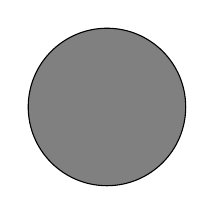
\begin{tikzpicture}
\filldraw[fill=gray] (0,0) circle[radius=1cm];
\tikzmark{b}{(-1,-1)}
\end{tikzpicture}
\end{frame}
\end{document}
